%
% 6.006 problem set 4 solutions template
%
\documentclass[12pt,twoside]{article}

\usepackage{amsmath}
\usepackage{color}
\usepackage{algorithm}
\usepackage{marvosym}
\usepackage[noend]{algpseudocode}

\usepackage{graphicx}
\usepackage{placeins}
\usepackage{hyperref}

\setlength{\oddsidemargin}{0pt}
\setlength{\evensidemargin}{0pt}
\setlength{\textwidth}{6.5in}
\setlength{\topmargin}{0in}
\setlength{\textheight}{8.5in}

\newcommand{\theproblemsetnum}{1}
\newcommand{\releasedate}{September 13, 2016}

\newcommand{\tabUnit}{3ex}
\newcommand{\tabT}{\hspace*{\tabUnit}}

\title{8.012 Problem Set 1}

\begin{document}
\delimitershortfall=-1pt

\centering
\textbf{8.012 Study Notes} \\ \vspace{5mm}
\textit{An Introduction To Mechanics 2nd. Edition, Kleppner \& Kolenkow}
\setlength{\parindent}{0pt}

\medskip

\hrulefill

\begin{flushleft}
\section*{Chapter 1: Vectors and Kinematics}
\subsection*{1.2: Vectors}

Vectors are represented using \textit{vector notation}. Vectors appear in \textbf{boldface}.
$$
\mathbf{F} = m\mathbf{a}
$$
Here, both $\mathbf{F}$ and $\mathbf{a}$ represent vector quantities. Occasionally, vectors are represented with an arrow, e.g., $\overrightarrow{A}$.
Vectors have both a \textit{length} and \textit{direction}. For two vectors to be equal, they must have identical length and direction.

The magnitude or size of a vector $\mathbf{A}$ is written $\left|\mathbf{A}\right|$, or simply $\mathit{A}$. If the length of a vector is one unit, we
call it a \textit{unit vector}, and label it with a caret. The vector of unit length parallel to $\mathbf{A}$ is $\mathbf{\hat{A}}$. We have that

$$
\mathbf{\hat{A}} = \frac{\mathbf{A}}{\mathit{A}}
$$

and

$$
\mathbf{A} = \mathit{A}\mathbf{\hat{A}}.
$$

\subsection*{1.3: The Algebra of Vectors}

\subsubsection*{1.3.1: Multiplying a Vector by a Scalar}

Multiplying a vector $\mathbf{A}$ by a scalar $\mathit{b}$ results in a new vector $\mathbf{C} = \mathit{b}\mathbf{A}$. If $\mathit{b} > 0$, then
$\mathbf{C}$ is parallel to $\mathbf{A}$, and its magnitude is $\mathit{b}$ times greater. thus $\mathbf{\hat{C}} = \mathbf{\hat{A}}$ and
$\mathit{C} = \mathit{b}\mathit{A}$. If $mathit{b} < 0$, then $\mathbf{C}$ is opposite in direction to $\mathbf{A}$, and its magnitude is
$\mathit{C} = \left|\mathit{b}\right|\mathit{A}$.

\subsubsection*{1.3.4: Algebraic Properties of Vectors}

Commutative law:

$$
\mathbf{A} + \mathbf{B} = \mathbf{B} + \mathbf{A}
$$

Associative law:

$$
\mathbf{A} + \left(\mathbf{B} + \mathbf{C}\right)= \left(\mathbf{B} + \mathbf{A}\right) + \mathbf{C}
$$
$$
\mathit{c}\left(\mathit{d}\mathbf{A}\right) = \left(\mathit{c}\mathit{d}\right)\mathbf{A}
$$

Distributive law:

$$
\mathit{c}\left(\mathbf{A} + \mathbf{B}\right) = \mathit{c}\mathbf{A} + \mathit{c}\mathbf{B}
$$
$$
\left(\mathit{c} + \mathit{d}\right)\mathbf{A} = \mathit{c}\mathbf{A} + \mathit{d}\mathbf{A}
$$

\subsection*{1.4: Multiplying Vectors}
\subsubsection*{1.4.1: Scalar Product (``Dot Product'')}

This type of multiplcation is called the \textit{scalar} product because its result is a scalar. It is written, e.g., $\mathbf{A}\cdot\mathbf{B}$.
It is defined as

$$
\mathbf{A}\cdot\mathbf{B} \equiv \mathit{A}\mathit{B}\cos{\theta}
$$

where $\theta$ is the angle between $\mathbf{A}$ and $\mathbf{B}$ when drawn tail to tail. Since $\mathit{B}\cos{\theta}$ is the projection of
$\mathbf{B}$ onto $\mathbf{A}$, it follows that

\begin{align*}
\mathbf{A}\cdot\mathbf{B} &= \mathit{A} \text{ times the projection of $\mathbf{B}$ onto $\mathbf{A}$} \\
& = \mathit{B} \text{ times the projection of $\mathbf{A}$ onto $\mathbf{B}$}
\end{align*}

Note that $\mathbf{A} \cdot \mathbf{A} = \left|\mathbf{A}\right|^{2} = \mathit{A}^2$, and $\mathbf{A}\cdot\mathbf{B} = \mathbf{B}\cdot\mathbf{A}$.
If $\mathbf{A}$ or $\mathbf{B}$ is zero, so is their dot product. Since $\cos{\pi/2} = 0$, the dot product of two nonzero vectors can also happen
to be zero, if the vectors are perpindicular.

\subsubsection*{1.4.2: Vector Product (``Cross Product'')}

This product is called the \textit{vector} product, since two vectors $\mathbf{A}$ and $\mathbf{B}$ are combined to form a third vector $\mathbf{C}$.
The symbol for vector product is a cross, lending the name \textit{cross} product:

$$
\mathbf{C} = \mathbf{A} \times \mathbf{B}
$$

The magnitude of the vector $\mathbf{C} = \mathbf{A} \times \mathbf{B}$ is defined as:

$$
\mathit{C} = \mathit{A}\mathit{B}\sin{\theta}
$$

where $\theta$ is the angle between $\mathbf{A}$ and $\mathbf{B}$ when they are drawn tail to tail. To eliminate any ambiguity, $\theta$ is always
chosen to be the angle smaller than $\pi$. Even if neither vector is zero, their cross product is zero if $\theta = 0$ or $\pi$; when the vectors are parallel
or antiparallel. It follows that for any vector $\mathbf{A}$,

$$
\mathbf{A} \times \mathbf{A} = 0.
$$

Two vectors $\mathbf{A}$ and $\mathbf{B}$ define a unique plane. The direction of $\mathbf{C}$ is defined to be perpindicular to this plane. $\mathbf{A}$, $\mathbf{B}$, and $\mathbf{C}$ form a \textit{right-hand triple}. If $\mathbf{A}$ lies on the $\mathit{x}$ axis and $\mathbf{B}$ lies toward the $\mathit{y}$ axis, then
$\mathbf{C}$ lies towards the positive $\mathit{z}$ axis. This definition leads towards the following consequence:

$$
\mathbf{B} \times \mathbf{A} = -\mathbf{A} \times \mathbf{B}
$$

The cross product is not commutative, but \textit{anticommutative}.

\subsection*{1.5: Components of a Vector}

We can uniquely define a vector in terms of its projections along axes of a coordinate system. Consider the vector $\mathbf{A}$ in the diagram below.

\begin{figure}[H]
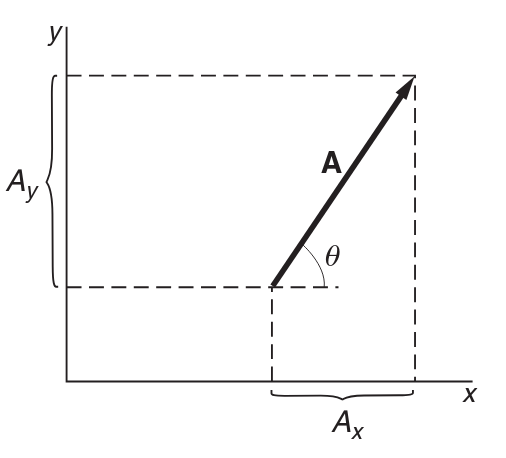
\includegraphics[scale=.4]{images/chapter1/image1.png}
\centering
\end{figure}

We have that the magnitude of $\mathbf{A}$ is $\sqrt{\mathit{A}_{x}^{2} + \mathit{A}_{y}^{2}}$, and the direction of $\mathbf{A}$ makes
$\theta = \arctan{\mathit{A}_{y}/\mathit{A}_{x}}$. Thus,

$$
\mathbf{A} = \left(\mathit{A}_{x}, \mathit{A}_{y}\right).
$$

Or in three dimensions:

$$
\mathbf{A} = \left(\mathit{A}_{x}, \mathit{A}_{y}, \mathit{A}_{z}\right).
$$

If two vectors are equal, then their corresponding componenets are equal.

Multiplication by a scalar is written

$$
\mathit{c}\mathbf{A} = \left(\mathit{c}\mathit{A}_{x}, \mathit{c}\mathit{A}_{y}, \mathit{c}\mathit{A}_{z}\right).
$$

Vector addition is written

$$
\mathbf{A} + \mathbf{B} = \left(\mathit{A}_{x} + \mathit{B}_{x}, \mathit{A}_{y} + \mathit{B}_{y}, \mathit{A}_{z} + \mathit{B}_{z} \right).
$$

By writing $\mathbf{A}$ and $\mathbf{B}$ as sums of vectors along each of the coordinate axes, it follows that

$$
\mathbf{A}\cdot\mathbf{B} = \mathit{A}_{x}\mathit{B}_{x} + \mathit{A}_{y}\mathit{B}_{y} + \mathit{A}_{z}\mathit{B}_{z}.
$$

\subsection*{1.6: Base Vectors}

Base vectors are a set of orthogonal unit vectors, one for each dimension. In the Cartesian coordinate system of three dimensions, we have unit vectors
$\mathbf{\hat{i}}$, $\mathbf{\hat{j}}$, and $\mathbf{\hat{k}}$, for axes $\mathit{x}$, $\mathit{y}$, and $\mathit{z}$, respectively.

\begin{figure}[H]
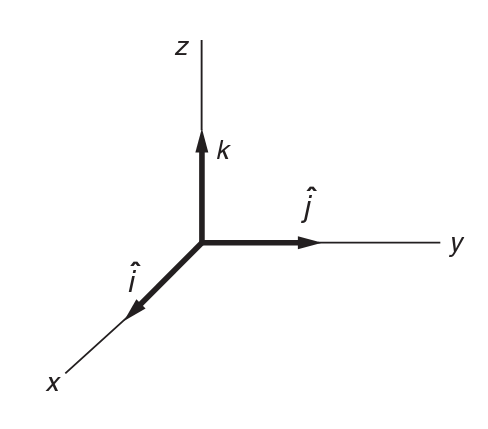
\includegraphics[scale=.4]{images/chapter1/image2.png}
\centering
\end{figure}

We have the following properties:

\begin{align*}
  \mathbf{\hat{i}}\cdot\mathbf{\hat{i}} &= \mathbf{\hat{j}}\cdot\mathbf{\hat{j}} = \mathbf{\hat{k}}\cdot\mathbf{\hat{k}} = 1 \\
  \mathbf{\hat{i}}\cdot\mathbf{\hat{j}} &= \mathbf{\hat{j}}\cdot\mathbf{\hat{k}} = \mathbf{\hat{k}}\cdot\mathbf{\hat{i}} = 0 \\
  \mathbf{\hat{i}}\times\mathbf{\hat{j}}&= \mathbf{\hat{k}} \\
  \mathbf{\hat{j}}\times\mathbf{\hat{k}}&= \mathbf{\hat{i}} \\
  \mathbf{\hat{k}}\times\mathbf{\hat{i}}&= \mathbf{\hat{j}} \\
\end{align*}

Any vector $\mathbf{A}$ can be written in terms of its components:

$$
\mathbf{A} = \mathit{A}_{x}\mathbf{\hat{i}} + \mathit{A}_{y}\mathbf{\hat{j}} + \mathit{A}_{z}\mathbf{\hat{k}}
$$

To find the component of a vector in any direction, take the dot product with a unit vector in that dimension.

The cross product of two vectors $\mathbf{A} = \left( \mathit{A}_{x}, \mathit{A}_{y}, \mathit{A}_{z} \right)$ and
$\mathbf{B} = \left( \mathit{B}_{x}, \mathit{B}_{y}, \mathit{B}_{z} \right)$ is

$$
\mathbf{A} \times \mathbf{B} = \left(\mathit{A}_{y}\mathit{B}_{z} - \mathit{A}_{z}\mathit{B}_{y} \right)\mathbf{\hat{i}} -
\left(\mathit{A}_{x}\mathit{B}_{z} - \mathit{A}_{z}\mathit{B}_{x} \right)\mathbf{\hat{j}} +
\left(\mathit{A}_{x}\mathit{B}_{y} - \mathit{A}_{y}\mathit{B}_{x} \right)\mathbf{\hat{k}}
$$

\subsection*{1.7: The Position Vector \textbf{r} and Displacement}

Consider an arbitrary point $\mathit{P}$ at coordinates $\left(\mathit{x}, \mathit{y}, \mathit{z}\right)$. Its position is written as

$$
\mathbf{r} = \left(\mathit{x}, \mathit{y}, \mathit{z}\right) = \mathit{x}\mathbf{\hat{i}} + \mathit{y}\mathbf{\hat{j}} + \mathit{z}\mathbf{\hat{k}}.
$$

If we move the point from $\mathit{x}_{1}, \mathit{y}_{1}, \mathit{z}_{1}$ to $\mathit{x}_{2}, \mathit{y}_{2}, \mathit{z}_{2}$, then the \textit{displacement}
defines a vector $\mathbf{S}$ with $\mathit{S}_{x} = \mathit{x}_{2} - \mathit{x}_{1}$, $\mathit{S}_{y} = \mathit{y}_{2} - \mathit{y}_{1}$, and
$\mathit{S}_{z} = \mathit{z}_{2} - \mathit{z}_{1}$. $\mathbf{S}$ points from the original position to the final position, and only encodes the \textit{relative}
position of each. Thus $\mathbf{S}$ is a \textit{true} vector: the values of the coordinates of its initial and final points depend on the coordinate system,
but $\mathbf{S}$ itself does not.

\begin{figure}[H]
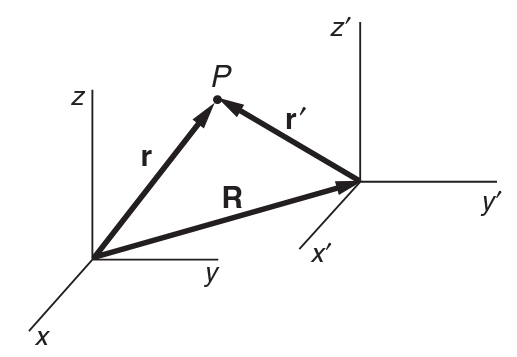
\includegraphics[scale=.4]{images/chapter1/image3.png}
\centering
\end{figure}

Consider the above figure. Vectors $\mathbf{r}$ and $\mathbf{r}'$ denote the position of the same point in space, but drawn in different coordinate systems.
$\mathbf{R}$ is the vector from the origin of the unprimed system to the origin of the primed coordinate system. We thus have
$\mathbf{r} = \mathbf{R} + \mathbf{r}'$, or equally, $\mathbf{r}' = \mathbf{r} - \mathbf{R}$.

\begin{figure}[H]
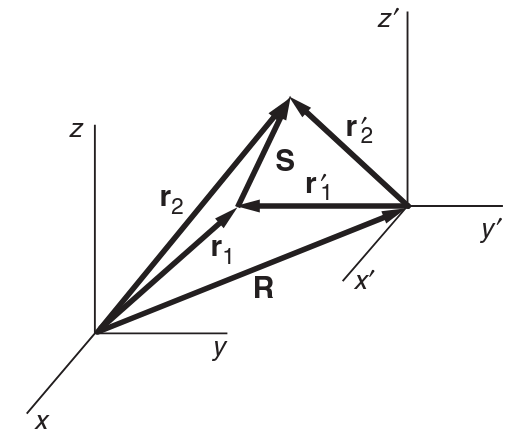
\includegraphics[scale=.4]{images/chapter1/image4.png}
\centering
\end{figure}

$\mathbf{S}$ above is a displacement vector. We show that it's independent of coordinate system chosen to represent it.

\begin{align*}
  \mathbf{S} &= \mathbf{r}_{2} - \mathbf{r}_{1} \\
             &= \left(\mathbf{R} + \mathbf{r}_{2}'\right) - \left(\mathbf{R} + \mathbf{r}_{1}'\right) \\
             &= \mathbf{r}_{2}' - \mathbf{r}_{1}'
\end{align*}

\subsection*{1.8: Velocity and Acceleration}
\subsubsection*{1.8.1: Motion in One Dimension}

Let $\mathit{x}$ be the value of the coordinate of a particle moving on a line. We assume a continuous record of position versus time.
The \textit{average velocity} $\mathit{\bar{v}}$ of the point between time $\textit{t}_{1}$ and $\textit{t}_{2}$ is defined by

$$
\mathit{\bar{v}} = \frac{\mathit{x}(\mathit{t}_{2}) - \mathit{x}(\mathit{t}_{1})}{\mathit{t}_{2} - \mathit{t}_{1}}.
$$

The \textit{instantaneous velocity} $\mathit{v}$ is the limit of the average velocity as the time interval approached zero.

$$
\mathit{v} = \lim_{\Delta\mathit{t} \rightarrow 0}\frac{\mathit{x}(\mathit{t} + \Delta\mathit{t}) - \mathit{x}(t)}{\Delta t}
$$

In the notation of Gottfried Leibniz, we write:

$$
v = \frac{dx}{dt}
$$

Newton would have written

$$
v = \dot{x}
$$

where the dot stands for $d/dt$. Newton's notation will only be used for derivatives with respect to time. The derivative of a function $f(x)$ can be
written $f'(x) \equiv df(x)/dx$.

Simililarly, the \textit{instantaneous acceleration} $a$ is

\begin{align*}
  a &= \lim_{\Delta\mathit{t} \rightarrow 0}\frac{\mathit{v}(\mathit{t} + \Delta\mathit{t}) - \mathit{v}(t)}{\Delta t} \\
    &= \frac{dv}{dt} = \dot{v}.
\end{align*}

Using $v = dx/dt$,

$$
a = \frac{d^2x}{dt^2} = \ddot{x}.
$$

The concept of speed may be useful. Speed $s$ is the magnitude of velocity: $s = |\mathbf{v}|$.

\subsubsection*{1.8.2: Motion in Several Dimensions}

Consider a particle moving in the $x-y$ plane. We know the particle's coordinate at every value of time. The instantaneous position of the particle
at some time $t_{1}$ is

$$
\mathbf{r}(t_{1}) = \left(x(t_{1}), y(t_{1})\right)
$$

or

$$
\mathbf{r}(t_{1}) = (x_{1},y_{1})
$$

The displacement of the particle between $t_1$ and $t_2$ is

$$
\mathbf{r}(t_2) - \mathbf{r}(t_1) = (x_2 - x_1, y_2 - y_1)
$$

The displacement of the particle during the interval $\Delta t$ is

$$
\Delta\mathbf{r} = \mathbf{r}(t + \Delta t) - \mathbf{r}(t).
$$

The above equation is equivalent to the two scalar equations

\begin{align*}
\Delta x &= x(t + \Delta t) - x(t) \\
\Delta y &= y(t + \Delta t) - y(t)
\end{align*}

The \textit{velocity} $\mathbf{v}$ of the particle as it moves is

\begin{align*}
  \mathbf{v} &= \lim_{\Delta t \rightarrow 0}\frac{\Delta \mathbf{r}}{\Delta t} \\
             &= \frac{d\mathbf{r}}{dt}
\end{align*}

which is equiavalent to the two scalar equiations

\begin{align*}
  v_x = &\lim_{\Delta t \rightarrow 0}\frac{\Delta x}{\Delta t} = \frac{dx}{dt} \\
  v_y = &\lim_{\Delta t \rightarrow 0}\frac{\Delta y}{\Delta t} = \frac{dy}{dt} \\
\end{align*}

Adding a third dimension, we tack on

$$
  v_z = \lim_{\Delta t \rightarrow 0}\frac{\Delta z}{\Delta t} = \frac{dz}{dt}
$$


Another approach to calculating velocity is to start with $\mathbf{r} = x\mathbf{\hat{i}} + y\mathbf{\hat{j}} + z\mathbf{\hat{k}}$, and differentiate.

$$
\frac{d\mathbf{r}}{dt} = \frac{d(x\mathbf{\hat{i}} + y\mathbf{\hat{j}} + z\mathbf{\hat{k}})}{dt}
$$

Since the base vectors are constant in time, we treat them as contants when we differentiate.

$$
\frac{d\mathbf{r}}{dt} = \frac{dx}{dt}\mathbf{\hat{i}} + \frac{dy}{dt}\mathbf{\hat{j}} + \frac{dz}{dt}\mathbf{\hat{k}}
$$

Acceleration $\mathbf{a}$ then, is

\begin{align*}
  \mathbf{a} &= \frac{d\mathbf{v}}{dt} = \frac{dv_x}{dt}\mathbf{\hat{i}} + \frac{dv_y}{dt}\mathbf{\hat{j}} + \frac{dv_z}{dt}\mathbf{\hat{k}} \\
  &= \frac{d^2\mathbf{r}}{dt}
\end{align*}

Let a particle undergo displacement $\Delta \mathbf{r}$ in time $\Delta t$. As $\Delta t \rightarrow 0$, $\Delta \mathbf{r}$ becomes tangent to trajectory.

\begin{align*}
  \Delta \mathbf{r} &\approx \frac{d\mathbf{r}}{dt}\Delta t \\
                    &= \mathbf{v}\Delta t
\end{align*}

becomes exact in the limit $\Delta t \rightarrow 0$. Thus the instantaneous velocity is at every point tangent to the trajectory.

\subsection*{1.9 Formal Solution of Kinematical Equations}

If acceleration is a known function of time, velocity can be found as

$$
\frac{d\mathbf{v}(t)}{dt} = \mathbf{a}(t)
$$

by integration with respect to time. Component-wise, this is

$$
\frac{dv_x}{dt}\mathbf{\hat{i}} + \frac{dv_y}{dt}\mathbf{\hat{j}} + \frac{dv_z}{dt}\mathbf{\hat{k}} = a_x\mathbf{\hat{i}} + a_y\mathbf{\hat{j}} + a_z\mathbf{\hat{k}}
$$

We can split this into individual components, e.g.,

$$
\frac{dv_x}{dt} = a_x
$$

If we know the velocity at some time $t_0$, we can integrate with respect to time to find the velocity at a later time $t_1$.

\begin{align*}
  \int_{v_0}^{v_1} dv_x &= \int_{t0}^{t_1} a_x dt \\
  v_x(t_1) - v_x(t_0) &= \int_{t_0}^{t_1} a_x(t)dt \\
\end{align*}
then

$$
v_x(t_1) = v_x(t_0) + \int_{t_0}^{t_1} a_x(t)dt
$$

Taking all components into account, we have

$$
\mathbf{v}(t_1) = \mathbf{v}(t_0) + \int_{t_0}^{t_1}\mathbf{a}(t)dt.
$$

The velocity at an arbitrary time $t$ is then

$$
\mathbf{v}(t) = \mathbf{v}_0 + \int_{t_0}^{t}\mathbf{a}(t')dt'.
$$

Position is the same. If

$$
\frac{d\mathbf{r}(t)}{dt} = \mathbf{v}(t)
$$

then

$$
\mathbf{r}(t) = \mathbf{r}_0 + \int_{t_0}^{t}\mathbf{v}(t')dt'.
$$

One important case is \textit{uniform acceleration}. If $\mathbf{a} = $ constant and $t_0 = 0$, we have

\begin{align*}
  \mathbf{v}(t) &= \mathbf{v}_0 + \mathbf{a}t \\
  \mathbf{r}(t) &= \mathbf{r}_0 + \int_{0}^t(\mathbf{v}_0 + \mathbf{a}t')dt'.
\end{align*}

or...

$$
\mathbf{r}(t) = \mathbf{r}_0 + \mathbf{v}_0t + \frac{1}{2}\mathbf{a}t^2.
$$

\subsection*{1.10: More about the Time Derivative of a Vector}

Consider a vector $\mathbf{A}(t)$ that changes with time. The change in $\mathbf{A}(t)$  over interval $t$ to $t + \Delta t$ is

$$
\Delta\mathbf{A} = \mathbf{A}(t + \Delta t) - \mathbf{A}(t)
$$

We define the time derivative of $\mathbf{A}$ by

$$
\frac{d\mathbf{A}}{dt} = \lim_{\Delta t \rightarrow 0}\frac{\mathbf{A}(t+\Delta t) - \mathbf{A}(t)}{\Delta t}
$$

\subsubsection*{1.11: Rotating Vectors}

If $d\mathbf{A}/dt$ is always perpindicular to $\mathbf{A}$, $\mathbf{A}$ must \textit{rotate}. This
cannot change its magnitude, since no component of the derivative is parallel to $\mathbf{A}$.

Suppose a vector $\mathbf{A}(t)$ has constant magnitude $A$, and the only way it can change in time
is by rotating. The direction of $d\mathbf{A}/dt$ is always perpindicular to $\mathbf{A}$. The magnitude
of $d\mathbf{A}/dt$ can be found by the following argument.

The change in $\mathbf{A}$ in the interbal $t$ to $t + \Delta t$ is

$$
\Delta \mathbf{A} = \mathbf{A}(t + \Delta t) - \mathbf{A}(t)
$$

Consider
\begin{figure}[H]
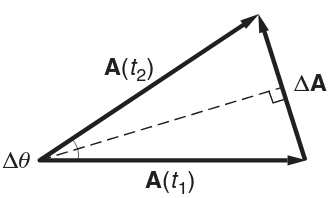
\includegraphics[scale=.4]{images/chapter1/image5.png}
\centering
\end{figure}

Then, using the angle $\Delta \theta$ from the image,

$$
|\Delta\mathbf{A}| = 2A\sin{\frac{\Delta \theta}{2}}
$$

For $\Delta\theta \ll 1$, $\sin{\Delta\theta/2} \approx \Delta\theta/2$. We have then

$$
|\Delta\mathbf{A}| = A\Delta\theta
$$

and thus

$$
\left|\frac{\Delta\mathbf{A}}{\Delta t}\right| \approx A\frac{\Delta\theta}{\Delta t}
$$

Taking the limit as $\Delta t \rightarrow 0$,

$$
\left|\frac{d\mathbf{A}}{dt}\right| = A\frac{d\theta}{dt}
$$

$d\theta/dt$ is called the \textit{angular speed} of $\mathbf{A}$.


\end{flushleft}
\end{document}

